\section{Evolutionary Computation}
\label{sec:evolutionary-computation}
Evolutionary computation is a family of techniques that uses mechanisms inspired by Darwin evolution theory to refine populations of candidate solutions to a given problem \cite{vikhar2016evolutionary}. It uses mechanisms such as reproduction, mutation, recombination and selection.

\begin{figure}[ht]
    \centering
    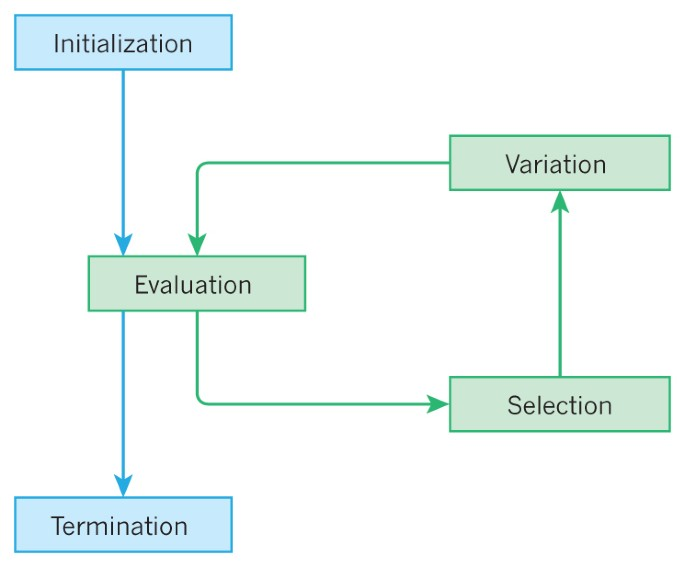
\includegraphics[width=0.4\textwidth]{images/Evolutionary_algorithms.jpg}
    \caption{Evolutionary Algorithm.}
\end{figure}

An evolutionary algorithm (EA) begins with the initialization of a population of randomly generated individuals. Each member of this population is then evaluated. 
The EA then uses a fitness-oriented procedure to select, breed, and mutate individuals to produce children which are then added to the population, replacing older individuals. 
One evaluation, selection, and variation (also known as breeding or reproduction) cycle is known as a generation. 
Successive generations continue to refine the population until time is exhausted or a sufficiently fit individual is discovered. 
Evolutionary computation methods include genetic algorithms (GA) and evolution strategies (ES), both of which are usually applied to the search of multidimensional parameter spaces; 
and genetic programming (GP) \cite{panait2005cooperative} \cite{vikhar2016evolutionary}.

Evolutionary algorithms can be used from learning agent to learn Solo Pong \cite{langdon2005evolutionary} and Pong \cite{mcbrien2020learning}.
It's also possible to designing neural networks through the use of NeuroEvolution \cite{stanley2019designing}, an evolutionary algorithm that optimize neural networks.
